\section{Approach}
\label{sec:approach}
\begin{figure}[t]
\centering
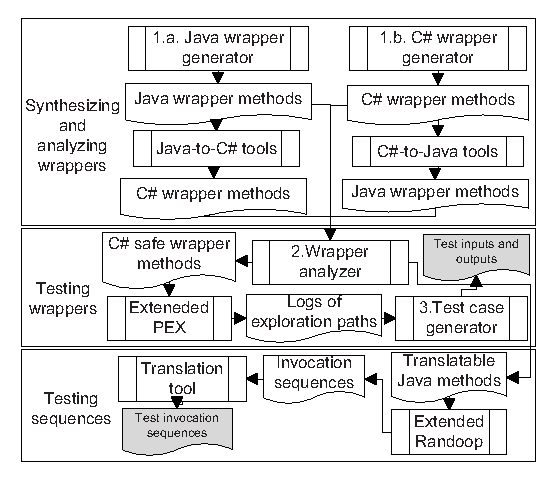
\includegraphics[scale=1,clip]{figure/approach.eps}\vspace*{-3ex}
 \caption{Overview of TeMAPI}\vspace*{-4ex}
 \label{fig:approach}
\end{figure}

Given a translation tool between Java and C\#, TeMAPI generates various test cases to reveal behavior differences of the tool's API mapping relations. Figure~\ref{fig:approach} shows the overview of TeMAPI. TeMAPI generates test cases not only to test mapping relations for a single API class but also for mapping relations of multiple API classes.


%-------------------------------------------------------------------
\subsection{Synthesizing Wrappers for Translation}
\label{sec:approach:generating}
Given a translation tool, TeMAPI first extracts its API mapping relations. To deal with different formats of translation tools as described in Section~\ref{sec:introduction}, TeMAPI does not extract API mapping relations directly from translation tools, but analyzes translated code for such relations. In particular, TeMAPI synthesizes one wrapper method for each field and each method given each constructor for each API class based on the reflection technique~\cite{maes1987concepts}. For static fields and static methods, TeMAPI uses the following rules to synthesize wrapper methods:

\textbf{Static fields.} Given a public static field \CodeIn{f} of a class \CodeIn{C} whose type is \CodeIn{T}, TeMAPI synthesizes a getter as follows:

\begin{CodeOut}\vspace*{-1ex}
\begin{alltt}
 public T TestGet|f.name||no|()\{ return C.f; \}
\end{alltt}
\end{CodeOut}\vspace*{-1ex}

If \CodeIn{f} is not a constant, TeMAPI synthesizes a setter as follows:

\begin{CodeOut}\vspace*{-1ex}
\begin{alltt}
 public void TestSet|f.name||no|(T v)\{ C.f = v; \}
\end{alltt}
\end{CodeOut}\vspace*{-1ex}

\textbf{Static methods.} Given a public static method \CodeIn{m(T1\ p1,\ldots,Tn\ pn)} of a class \CodeIn{C} whose return type is \CodeIn{Tm}, TeMAPI synthesizes a wrapper method as follows:

\begin{CodeOut}\vspace*{-1ex}
\begin{alltt}
 public Tm Test|m.name||no|(T1\ m1,\ldots, Tn\ mn)\{
   return C.m(m1,\ldots, mn); \}
\end{alltt}
\end{CodeOut}\vspace*{-1ex}

When TeMAPI synthesizes wrapper methods for non-static fields or methods, it takes constructor into considerations:

\textbf{Non-static fields.} Given a public non-static field \CodeIn{f} of a class \CodeIn{C} whose type is \CodeIn{T}, TeMAPI synthesizes a getter for each constructor \CodeIn{C(T1\ p1,\ldots, Tn\ pn)} of \CodeIn{C} as follows:

\begin{CodeOut}\vspace*{-1ex}
\begin{alltt}
 public T TestGet|f.name||no|(T1\ c1,\ldots, Tn\ cn)\{
    C obj = new C(c1,\ldots, cn);
    return obj.f; \}
\end{alltt}
\end{CodeOut}\vspace*{-1ex}

If \CodeIn{f} is not a constant, TeMAPI synthesizes a setter as follows:

\begin{CodeOut}\vspace*{-1ex}
\begin{alltt}
 public void TestSet|f.name||no|(T1\ c1,\ldots, Tn\ cn)\{
   C obj = new C(c1,\ldots, cn);
   obj.f = v; \}
\end{alltt}
\end{CodeOut}\vspace*{-1ex}

Here, ``\CodeIn{|f.name|}'' denotes the name of \CodeIn{f}, and ``\CodeIn{|no|}'' denotes the corresponding number of synthesized wrapper method.

\textbf{Non-static methods.} Given a public non-static method \CodeIn{m(T1\ p1,\ldots,Tn\ pn)} of a class \CodeIn{C} whose return type is \CodeIn{Tm}, TeMAPI synthesizes a wrapper method for each constructor \CodeIn{C(Tv\ pv,\ldots, Tt\ pt)} of \CodeIn{C} as follows:

\begin{CodeOut}\vspace*{-1ex}
\begin{alltt}
 public Tm Test|m.name||no|(T1\ m1,\ldots, Tn\ mn,
                            Tv cv, \ldots, Tt ct)\{
   C obj = new C(cv,\ldots, ct);
   return obj.m(m1,\ldots, mn); \}
\end{alltt}
\end{CodeOut}\vspace*{-1ex}

Here, ``\CodeIn{|m.name|}'' denotes the name of \CodeIn{m(T1\ p1,\ldots,Tn\ pn)}.

TeMAPI put all synthesized wrapper methods for one API class $C$ into one synthesized class. For a Java-to-C\# tools, TeMAPI synthesizes wrapper methods in Java as shown by the solid line in Figure~\ref{fig:approach}, and for a C\#-to-Java tools, TeMAPI synthesizes wrapper methods in C\# as shown by the dotted line in Figure~\ref{fig:approach}. When synthesizing, TeMAPI ignores generic methods, and when synthesizing for C\# API classes, TeMAPI ignores \CodeIn{unsafe} methods, \CodeIn{delegate} methods, and methods whose parameters are marked as \CodeIn{out} or \CodeIn{ref} besides generic methods. Java does not have corresponding keywords, so existing translation tools typically do not translate the preceding methods. After wrappers are synthesized, we translate them using a translation tool under analysis.

After synthesized code is translated, TeMAPI parses translated code to filter out wrapper methods with compilation errors. We use \emph{safe wrappers} to refer to the remaining wrapper methods. To identify wrapper methods with compilation errors, TeMAPI extends Visual Studio and Eclipse's Java compiler for C\# and Java code, respectively.
%For Java-to-C\# tools, TeMAPI extends Visual Studio through its automation and extensibility interfaces to parse translated C\# wrapper methods and removes those translated methods with compilation errors. We refer to the remaining C\# wrapper methods as safe wrappers. For C\#-to-Java tools, TeMAPI extends the Eclipse's Java compiler to parse translated Java wrapper methods and removes those translated methods with compilation errors. We refer to the synthesized C\# wrapper methods that can be translated into Java without compilation errors as safe wrappers. 
Since wrappers reveal behaviors of a given class at the finest level and expose interfaces for inputs and outputs, TeMAPI further uses safe wrappers to test behavior differences for single API classes (Section~\ref{sec:approach:single}). Comparing safe wrappers with synthesized wrappers, TeMAPI can extract the list of translatable API elements for a given translation tool. Using the list, TeMAPI further tests behavior difference for multiple API classes (Section~\ref{sec:approach:sequence}).


%for validate API mapping relations of the translation tool. To achieve this, TeMAPI first remove all translated methods with compilation errors. For translated methods in Java, TeMAPI implements a Eclipse plug-in that uses on Eclipse JDT compiler\footnote{\url{http://www.eclipse.org/jdt/}} for the list of compilation errors. For translated methods in C\#, TeMAPI implements a Visual Studio.Net add-in to retrieve the list of compilation errors from the error-list view of Visual Studio.Net. Both Eclipse JDT compiler and Visual Studio.Net cannot list all methods with compilation errors in a single build. After each iteration of removing methods, TeMAPI re-build these methods until it removes all methods with compilation errors.
%
%After methods with compilation errors are removed, TeMAPI compares synthesized code with translated code for the validate API mapping relations of a translation tool. Based on translated code and validate API mapping, TeMAPI removes synthesized methods whose corresponding translated methods have compilation errors. We refer to those removing wrapper methods as safe methods.


%-----------------------------------------------------------------
\subsection{Testing Single API Classes}
\label{sec:approach:single}
As shown in Figures~\ref{fig:db4ojava} and~\ref{fig:db40net}, translation tools can translate one API class in one language into one class in another language. To detect behavior differences that involve single classes, TeMAPI extends Pex~\cite{tillmann2008pex}, so that it generates test cases for safe wrapper methods for each API class in C\#. Pex~\cite{tillmann2008pex} is a white-box test generation tool for .NET based on dynamic symbolic execution. Basically, Pex repeatedly executes a method under test, so that it explores all feasible paths of the method. 
%To reduce the efforts to explore paths, Pex leverage various exploration strategies. For example, Xie \emph{et al.}~\cite{xie09:fitness} propose a search strategy called Fitnex that uses state-dependent fitness values to guide path exploration of Pex. 
For each API class, TeMAPI leverages Pex to explore paths of each its safe wrapper, and records the inputs and the corresponding output when exploring. Based on recorded inputs and outputs, TeMAPI generates Java test cases to ensure each wrapper methods produce the same output give the same inputs. To check equivalence of  outputs, TeMAPI checks whether their values are equal for primitive types and arrays, and checks whether each mapped fields are equal for objects. For example, TeMAPI records that given an empty object, the \CodeIn{testappend175nm} wrapper method in C\# return a \CodeIn{StringBuilder} object whose \CodeIn{Capacity} field is 16 and \CodeIn{Length} field is 13, so TeMAPI generates a test case for the corresponding Java wrapper method as follows:

\begin{CodeOut}\vspace*{-1ex}
\begin{alltt}
public void testappend175nm122()\{
  sketch.Test_java_lang_StringBuffer obj =
      new sketch.Test_java_lang_StringBuffer();
  Object m0 = new Object();
  StringBuffer out = obj.testappend175nm(m0);
  Assert.assertEquals(16, out.capacity());	
  Assert.assertEquals(13, out.length());
\}
\end{alltt}
\end{CodeOut}\vspace*{-2ex}

This test case fails, since here the \CodeIn{capacity()} method returns 34 and the \CodeIn{length()} method returns 24. Thus, TeMAPI detects two behavior differences between the \CodeIn{java.lang.StringBuffer} class in Java and the \CodeIn{System.Text.StringBuilder} class in C\#.


We notice that when Pex explores a path with some specific inputs, the method under exploration throws exceptions.
For example, during exploring the \CodeIn{TestvalueOf61sm} wrapper method, TeMAPI records that given a \CodeIn{null} input, the method throws \CodeIn{Null- ReferenceException}, so it generates a test case to ensure the corresponding Java wrapper method also throws a mapped exception. To generate the test case, TeMAPI first finds the corresponding exceptions in Java by analyzing translated wrapper methods with synthesized ones. In this example, TeMAPI finds that the \CodeIn{NullReferenceException} class in C\# is mapped to the \CodeIn{Null- PointerException} class in Java with respect to the API mapping relations of Java2CSharp, so it generates a Java test case as follows:

\begin{CodeOut}\vspace*{-1ex}
\begin{alltt}
 public void testvalueOf61sm3()\{
   try\{
     sketch.Test_java_lang_String obj =
           new sketch.Test_java_lang_String();
     java.lang.Object m0 = null;
     obj.testvalueOf61sm(m0);
   \}catch(java.lang.NullPointerException e)\{
     Assert.assertTrue(true);
     return;
   \}
   Assert.assertTrue(false); \}
\end{alltt}
\end{CodeOut}\vspace*{-1ex}

This test case fails since the \CodeIn{testvalueOf61sm} method does not throw any exceptions given a null input.
From this failed Java test case, TeMAPI detects the behavior difference between the \CodeIn{java. lang.String.valueOf(Object)} method in Java and the \CodeIn{System. Object.ToString()} method in C\#, since the preceding two wrapper methods are for the two API methods only.
\begin{table}[t]
\centering
\begin{SmallOut}
\begin {tabular} {|c|l|c|c|c|c|c|c|}
 \hline
\textbf{Name}& \textbf{Version}& \textbf{Provider} &\textbf{Description}\\
\hline
Java2CSharp  &  1.3.4 & IBM (ILOG) & Java to C\# \\
\hline
JLCA         &  3.0   & Microsoft  & Java to C\# \\
\hline
sharpen      &  1.4.6 & db4o       & Java to C\# \\
\hline
Net2Java     &  1.0   & NetBean    &  C\# to Java\\
\hline
converter    &  1.6   & Tangible   &  C\# to Java\\
\hline
\end{tabular}\vspace*{-2ex}
\Caption{Subject tools} \label{table:subjects}
\end{SmallOut}\vspace*{-2ex}
\end{table}
%-----------------------------------------------------------
\subsection{Testing Multiple Classes}
\label{sec:approach:sequence}
As shown in Figure~\ref{fig:javacode} and Figure~\ref{fig:codeJLCA}, translation tools can translate one invocation to invocation sequences that involve multiple classes. As each wrapper method uses only one field or one method of a given API class, it loses some behavior differences that involve multiple classes. To detect such differences, TeMAPI first extracts a list of translatable API methods for the translation tool under analysis. In particular, if a translation tool translates a wrapper method into the other language, TeMAPI considers all API methods within the wapper method as translatable API methods if the migration tool. For example, as shown in Section~\ref{sec:example}, JLCA translates the \CodeIn{testskip24nm} wrapper method into the other language, so TeMAPI its wrapped \CodeIn{BufferedInputStream(InputStream)} constructor and the \CodeIn{BufferedInputStream.skip(long)} method into translatable API methods of JLCA.

After translatable API methods of a translation tool are extracted, TeMAPI extends Randoop~\cite{pacheco2007feedback} to generate invocations sequences of API methods. Randoop randomly generates test cases based on already generated test cases in a feedback-directed manner, and it has both a Java version and a C\# version. When generating test cases, TeMAPI limits its search scope within translatable API methods only. After test cases are generated, TeMAPI runs these test cases, and removes all failed test cases. We translate the remaining test case into the other language using the translation tool under analysis. If translated code has the same behaviors, translated test cases should also get passed. If not, TeMAPI detects a behavior difference. As invocation sequences typically use multiple classes, such difference can involve multiple classes. Section~\ref{sec:example} shows a detected behavior difference through the \CodeIn{test413} test case.


%In the final step, TeMAPI generates test cases to detect behavior differences of API mapping relations. An alternative approach is to use existing test cases in two languages. For example, lucene\footnote{\url{http://lucene.apache.org}} has both a Java version and a C\# version. It is feasible to use these test cases to reveal some behavior differences, but such test cases typically cover only a small set of APIs. Some test suites such as Java Compatibility Kit (JCK)\footnote{\url{http://jck.dev.java.net}} cover most APIs of a language. However, translating such a test suite from one language into another language may introduce many compilation errors and defects. A test method may use many APIs, so even if the API under test can be translated correctly, the test method cannot be translated correctly since other APIs are not mapped. As a result, we choose to translating


%\subsubsection{Translating Existing Test Cases}
%\label{sec:approach:behavior:jck}
%
%Each generated wrapper method uses only one fields or methods provided by API libraries, and may lose some complicated behaviors even if test cases satisfy the round-trip criterion. To test those complicated behaviors, we introduce JCK that covers many complicated behaviors of Java APIs. JCK is a test suite provided by Sun to ensure compatibility of Java platforms, and it covers most standard APIs of J2SE. However, JCK implements many internal classes to collect the results of executed test cases. If a translation tool cannot correctly translate one of these classes, all translated test cases may have compilation errors or defects. In addition, JCK is released under read-only source license\footnote{\url{http://tinyurl.com/33x9fo6}}, so many such internal classes are not shipped and it has many compilation errors. To increase the chance of migrating JCK, TeMAPI first replaces those internal classes with the classes of Java. For example, one test method for \CodeIn{java.io.File.delete()} in JCK is as follows:
%
%\begin{CodeOut}%\vspace*{-2ex}
%\begin{alltt}
%  public Status File0037()\{
%    String testCaseID = "File0037";
%    ...
%    FileRT method = new FileRT(testCaseID) \{
%     public Status run() \{
%       File f = null;
%       f = new File(workdir, testCaseID);
%       ...
%       if (f.delete()) \{ // Try to delete
%         if (!f.exists()) \{ // Does it exist?
%           return Status.passed("OKAY");
%         \}else\{
%            return Status.failed(...);
%         \}
%       else\{
%           return Status.failed(...);
%       \}
%    \}
%     return AllPermissionSM.testRun(...);
%  \}
%\end{alltt}
%\end{CodeOut}
%
%After the preceding three steps, TeMAPI further replaces the statement starts with \CodeIn{FileRT} with the body of the \CodeIn{run} method, and removes the last statement. The translated code is as follows:
%
%\begin{CodeOut}%\vspace*{-2ex}
%\begin{alltt}
%  public void File0037()\{
%    String testCaseID = "File0037";
%    ...
%    File f = null;
%    f = new File(workdir, testCaseID);
%    ...
%    if (f.delete()) \{ // Try to delete
%      if (!f.exists()) \{ // Does it exist?
%        Assert.assertTrue(true);
%        return;
%     \}else\{
%        Assert.fail();
%        return;
%     \}
%   else\{
%       Assert.fail();
%       return;
%   \}
%  \}
%\end{alltt}
%\end{CodeOut}
%
%Compared with the original test method in JCK, the translated method does not use the three internal classes: \CodeIn{Status}, \CodeIn{FileRT}, and \CodeIn{AllPermissionSM}.
%
%After the preceding process, for a translation tool, TeMAPI further removes methods that use any APIs outside its defined mapping relations. The remaining methods can be translated from Java to other languages since it does not use any APIs outside of the translation tool.


